\section{Coinbase Exchange}

To simulate a real world security, high frequency LOB data of cryptocurrency securities is collected from Coinbase Pro. Coinbase Pro (formerly known as Global Digital Asset Exchange or GDAX) is the advanced trading platform of the Coinbase, which is an exchange founded in 2012 that brokers trades of many cryptocurrencies as well as fiat-currency to cryptocurrency exchanges. Major cryptocurrencies that are traded on Coinbase Pro include Bitcoin, Bitcoin Cash, Ethereum, Ethereum Classic, and Litecoin, while fiat-currencies are typically the USD or Euro. As of December 2018, Coinbase Pro has a total daily trading volume of about \$70 million (\cite{L1}). Coinbase Pro was chosen as the data source since it has readily accessible real-time LOB data that is freely available to developers from its API. It also features relatively liquid securities with large trading volumes. 

Although the LOB dynamics of the securities modelled in this paper may not entirely reflect those of securities from other exchanges such as stocks, futures, etc., the methodology in this paper is adaptable to the LOB data of any type of any relatively liquid security. The trading rules of Coinbase Pro are representative of most exchanges around the world. Coinbase Pro allows limit and market orders with time priority matching. It also allows stop orders, which is an order to place a limit or market order when the price of the security reaches a specified price. Coinbase Pro also differentiates between “maker” and “taker” orders. Taker orders are orders that fill immediately (such as market orders) and maker orders are orders that do not fill immediately and thus populate the LOB (such as limit orders). The fee structure, which is up to 0.3\% for taker orders depending on the volume and 0\% for maker orders encourages market making and therefore increases liquidity of the market. There are also rules to prevent self-trade, which is when the same trader acts as both the maker and taker for a trade. In addition, there are minimum and maximum orders for each security. Full trading rules for Coinbase Pro can be found on its website (\cite{L2}).

\section{Data Collection}
Data is collected through the Coinbase Pro API using a Python library called CoPrA, which is an asynchronous web socket client (\cite{L3}). Specifically, the ``level2" channel is used, which first provides a snapshot of the LOB. It also provides updates at every position of the LOB whenever an order happens. See listing \ref{data-collection-code} for the code written for data collection. Using these updates, an internal LOB is maintained for use during data analysis. Data was collected for several days in the months of December and January for all the level2 updates on the ETC-USD LOB (Ethereum Classic for USD), which has a daily trading volume of around \$2 million (\cite{L1}). The initial LOB is shown in Figure \ref{fig:12_30_18_LOB_pic}. The 10 best bids and asks are shown, which is where the vast majority of updates are made, but updates are also recorded for prices farther from the reference price.

\begin{figure}[t]
\begin{center}
\caption{LOB Sample}
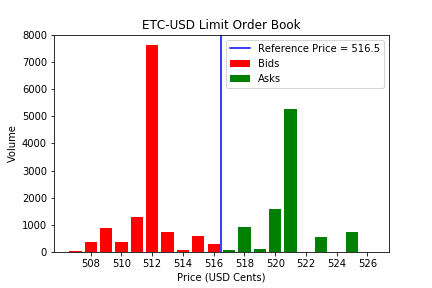
\includegraphics[width=\textwidth]{Figures/12_30_18_LOB.png}
\label{fig:12_30_18_LOB_pic}
\end{center}
\end{figure}

This LOB is typical for ETC-USD, with most of the positions near the reference price filled. The bid and ask sides are relatively balanced, meaning that the reference price is stable. This pattern is not always the case, as the bid or ask side could have significantly more volume when the price shifts. An sample of updates are shown in Figure \ref{fig:12_30_18_Updates}. Updates consist of the side, price, amount, and time. An update with an amount ``0" means that the liquidity at the price is completely consumed. As can be seen, the updates are given to the nearest millisecond and the majority of the updates occur near the reference price. The remainder of the thesis is based on the analysis of trading data from December 28-30, 2018 that includes almost all the trades of ETC-USD in that time period (there small gaps of a few minutes due to starting and stopping data collection).

\begin{figure}[t]
\begin{center}
\caption{First 20 LOB Updates for December 30, 2018}
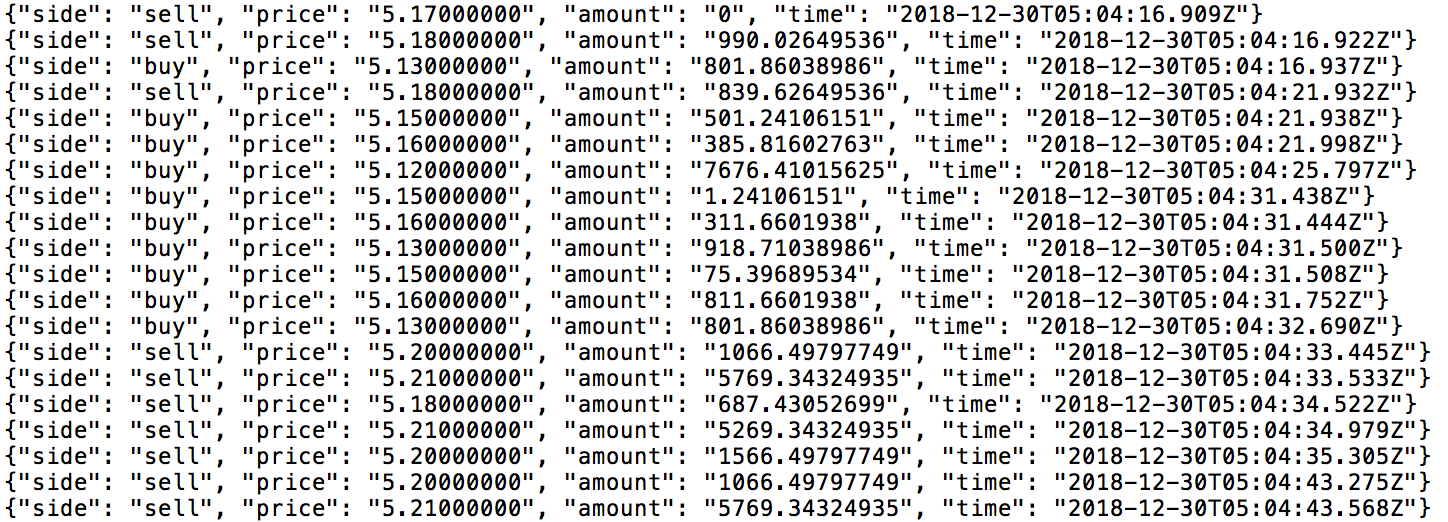
\includegraphics[width=\textwidth]{Figures/12_30_18_Updates.png}
\label{fig:12_30_18_Updates}
\end{center}
\end{figure}


